% Options for packages loaded elsewhere
\PassOptionsToPackage{unicode}{hyperref}
\PassOptionsToPackage{hyphens}{url}
\PassOptionsToPackage{dvipsnames,svgnames,x11names}{xcolor}
%
\documentclass[
  letterpaper,
  DIV=11,
  numbers=noendperiod]{scrartcl}

\usepackage{amsmath,amssymb}
\usepackage{iftex}
\ifPDFTeX
  \usepackage[T1]{fontenc}
  \usepackage[utf8]{inputenc}
  \usepackage{textcomp} % provide euro and other symbols
\else % if luatex or xetex
  \usepackage{unicode-math}
  \defaultfontfeatures{Scale=MatchLowercase}
  \defaultfontfeatures[\rmfamily]{Ligatures=TeX,Scale=1}
\fi
\usepackage{lmodern}
\ifPDFTeX\else  
    % xetex/luatex font selection
\fi
% Use upquote if available, for straight quotes in verbatim environments
\IfFileExists{upquote.sty}{\usepackage{upquote}}{}
\IfFileExists{microtype.sty}{% use microtype if available
  \usepackage[]{microtype}
  \UseMicrotypeSet[protrusion]{basicmath} % disable protrusion for tt fonts
}{}
\makeatletter
\@ifundefined{KOMAClassName}{% if non-KOMA class
  \IfFileExists{parskip.sty}{%
    \usepackage{parskip}
  }{% else
    \setlength{\parindent}{0pt}
    \setlength{\parskip}{6pt plus 2pt minus 1pt}}
}{% if KOMA class
  \KOMAoptions{parskip=half}}
\makeatother
\usepackage{xcolor}
\setlength{\emergencystretch}{3em} % prevent overfull lines
\setcounter{secnumdepth}{-\maxdimen} % remove section numbering
% Make \paragraph and \subparagraph free-standing
\makeatletter
\ifx\paragraph\undefined\else
  \let\oldparagraph\paragraph
  \renewcommand{\paragraph}{
    \@ifstar
      \xxxParagraphStar
      \xxxParagraphNoStar
  }
  \newcommand{\xxxParagraphStar}[1]{\oldparagraph*{#1}\mbox{}}
  \newcommand{\xxxParagraphNoStar}[1]{\oldparagraph{#1}\mbox{}}
\fi
\ifx\subparagraph\undefined\else
  \let\oldsubparagraph\subparagraph
  \renewcommand{\subparagraph}{
    \@ifstar
      \xxxSubParagraphStar
      \xxxSubParagraphNoStar
  }
  \newcommand{\xxxSubParagraphStar}[1]{\oldsubparagraph*{#1}\mbox{}}
  \newcommand{\xxxSubParagraphNoStar}[1]{\oldsubparagraph{#1}\mbox{}}
\fi
\makeatother

\usepackage{color}
\usepackage{fancyvrb}
\newcommand{\VerbBar}{|}
\newcommand{\VERB}{\Verb[commandchars=\\\{\}]}
\DefineVerbatimEnvironment{Highlighting}{Verbatim}{commandchars=\\\{\}}
% Add ',fontsize=\small' for more characters per line
\usepackage{framed}
\definecolor{shadecolor}{RGB}{241,243,245}
\newenvironment{Shaded}{\begin{snugshade}}{\end{snugshade}}
\newcommand{\AlertTok}[1]{\textcolor[rgb]{0.68,0.00,0.00}{#1}}
\newcommand{\AnnotationTok}[1]{\textcolor[rgb]{0.37,0.37,0.37}{#1}}
\newcommand{\AttributeTok}[1]{\textcolor[rgb]{0.40,0.45,0.13}{#1}}
\newcommand{\BaseNTok}[1]{\textcolor[rgb]{0.68,0.00,0.00}{#1}}
\newcommand{\BuiltInTok}[1]{\textcolor[rgb]{0.00,0.23,0.31}{#1}}
\newcommand{\CharTok}[1]{\textcolor[rgb]{0.13,0.47,0.30}{#1}}
\newcommand{\CommentTok}[1]{\textcolor[rgb]{0.37,0.37,0.37}{#1}}
\newcommand{\CommentVarTok}[1]{\textcolor[rgb]{0.37,0.37,0.37}{\textit{#1}}}
\newcommand{\ConstantTok}[1]{\textcolor[rgb]{0.56,0.35,0.01}{#1}}
\newcommand{\ControlFlowTok}[1]{\textcolor[rgb]{0.00,0.23,0.31}{\textbf{#1}}}
\newcommand{\DataTypeTok}[1]{\textcolor[rgb]{0.68,0.00,0.00}{#1}}
\newcommand{\DecValTok}[1]{\textcolor[rgb]{0.68,0.00,0.00}{#1}}
\newcommand{\DocumentationTok}[1]{\textcolor[rgb]{0.37,0.37,0.37}{\textit{#1}}}
\newcommand{\ErrorTok}[1]{\textcolor[rgb]{0.68,0.00,0.00}{#1}}
\newcommand{\ExtensionTok}[1]{\textcolor[rgb]{0.00,0.23,0.31}{#1}}
\newcommand{\FloatTok}[1]{\textcolor[rgb]{0.68,0.00,0.00}{#1}}
\newcommand{\FunctionTok}[1]{\textcolor[rgb]{0.28,0.35,0.67}{#1}}
\newcommand{\ImportTok}[1]{\textcolor[rgb]{0.00,0.46,0.62}{#1}}
\newcommand{\InformationTok}[1]{\textcolor[rgb]{0.37,0.37,0.37}{#1}}
\newcommand{\KeywordTok}[1]{\textcolor[rgb]{0.00,0.23,0.31}{\textbf{#1}}}
\newcommand{\NormalTok}[1]{\textcolor[rgb]{0.00,0.23,0.31}{#1}}
\newcommand{\OperatorTok}[1]{\textcolor[rgb]{0.37,0.37,0.37}{#1}}
\newcommand{\OtherTok}[1]{\textcolor[rgb]{0.00,0.23,0.31}{#1}}
\newcommand{\PreprocessorTok}[1]{\textcolor[rgb]{0.68,0.00,0.00}{#1}}
\newcommand{\RegionMarkerTok}[1]{\textcolor[rgb]{0.00,0.23,0.31}{#1}}
\newcommand{\SpecialCharTok}[1]{\textcolor[rgb]{0.37,0.37,0.37}{#1}}
\newcommand{\SpecialStringTok}[1]{\textcolor[rgb]{0.13,0.47,0.30}{#1}}
\newcommand{\StringTok}[1]{\textcolor[rgb]{0.13,0.47,0.30}{#1}}
\newcommand{\VariableTok}[1]{\textcolor[rgb]{0.07,0.07,0.07}{#1}}
\newcommand{\VerbatimStringTok}[1]{\textcolor[rgb]{0.13,0.47,0.30}{#1}}
\newcommand{\WarningTok}[1]{\textcolor[rgb]{0.37,0.37,0.37}{\textit{#1}}}

\providecommand{\tightlist}{%
  \setlength{\itemsep}{0pt}\setlength{\parskip}{0pt}}\usepackage{longtable,booktabs,array}
\usepackage{calc} % for calculating minipage widths
% Correct order of tables after \paragraph or \subparagraph
\usepackage{etoolbox}
\makeatletter
\patchcmd\longtable{\par}{\if@noskipsec\mbox{}\fi\par}{}{}
\makeatother
% Allow footnotes in longtable head/foot
\IfFileExists{footnotehyper.sty}{\usepackage{footnotehyper}}{\usepackage{footnote}}
\makesavenoteenv{longtable}
\usepackage{graphicx}
\makeatletter
\def\maxwidth{\ifdim\Gin@nat@width>\linewidth\linewidth\else\Gin@nat@width\fi}
\def\maxheight{\ifdim\Gin@nat@height>\textheight\textheight\else\Gin@nat@height\fi}
\makeatother
% Scale images if necessary, so that they will not overflow the page
% margins by default, and it is still possible to overwrite the defaults
% using explicit options in \includegraphics[width, height, ...]{}
\setkeys{Gin}{width=\maxwidth,height=\maxheight,keepaspectratio}
% Set default figure placement to htbp
\makeatletter
\def\fps@figure{htbp}
\makeatother

\usepackage{booktabs}
\usepackage{longtable}
\usepackage{array}
\usepackage{multirow}
\usepackage{wrapfig}
\usepackage{float}
\usepackage{colortbl}
\usepackage{pdflscape}
\usepackage{tabu}
\usepackage{threeparttable}
\usepackage{threeparttablex}
\usepackage[normalem]{ulem}
\usepackage{makecell}
\usepackage{xcolor}
\KOMAoption{captions}{tableheading}
\makeatletter
\@ifpackageloaded{caption}{}{\usepackage{caption}}
\AtBeginDocument{%
\ifdefined\contentsname
  \renewcommand*\contentsname{Table of contents}
\else
  \newcommand\contentsname{Table of contents}
\fi
\ifdefined\listfigurename
  \renewcommand*\listfigurename{List of Figures}
\else
  \newcommand\listfigurename{List of Figures}
\fi
\ifdefined\listtablename
  \renewcommand*\listtablename{List of Tables}
\else
  \newcommand\listtablename{List of Tables}
\fi
\ifdefined\figurename
  \renewcommand*\figurename{Figure}
\else
  \newcommand\figurename{Figure}
\fi
\ifdefined\tablename
  \renewcommand*\tablename{Table}
\else
  \newcommand\tablename{Table}
\fi
}
\@ifpackageloaded{float}{}{\usepackage{float}}
\floatstyle{ruled}
\@ifundefined{c@chapter}{\newfloat{codelisting}{h}{lop}}{\newfloat{codelisting}{h}{lop}[chapter]}
\floatname{codelisting}{Listing}
\newcommand*\listoflistings{\listof{codelisting}{List of Listings}}
\makeatother
\makeatletter
\makeatother
\makeatletter
\@ifpackageloaded{caption}{}{\usepackage{caption}}
\@ifpackageloaded{subcaption}{}{\usepackage{subcaption}}
\makeatother

\ifLuaTeX
  \usepackage{selnolig}  % disable illegal ligatures
\fi
\usepackage{bookmark}

\IfFileExists{xurl.sty}{\usepackage{xurl}}{} % add URL line breaks if available
\urlstyle{same} % disable monospaced font for URLs
\hypersetup{
  pdftitle={Project Part 3},
  pdfauthor={Liam Quach, Dylan Li, and Brendan Callender},
  colorlinks=true,
  linkcolor={blue},
  filecolor={Maroon},
  citecolor={Blue},
  urlcolor={Blue},
  pdfcreator={LaTeX via pandoc}}


\title{Project Part 3}
\author{Liam Quach, Dylan Li, and Brendan Callender}
\date{}

\begin{document}
\maketitle


\subsection{Part I: Proposal and Data
Assembly}\label{part-i-proposal-and-data-assembly}

\subsubsection{Background}\label{background}

The English Premier League (EPL) is the top tier of professional
football (soccer) in England and is considered one of the most popular
and competitive leagues in the world. The league is made up of twenty
clubs (teams) that compete over a season for the Premier League title.
Each year, three new clubs are promoted from the second division based
on the previous year's results. These promoted teams replace the bottom
three teams from the premier league for the previous year.

Over the course of a season, each team plays 38 matches per season,
facing every other team twice---once at home and once away. Teams are
rewarded points as follows: 3 points for a win, 1 points for a draw, and
0 points for a loss. The team with the most points at the end of the
38-game season is crowned as Premier League Champions.

For our project, we are interested in seeing which factors are
associated of higher or lower point totals in the English Premier
league. To address our main research question, we have collected data
from the English Premier League for seasons between 2017 and 2023. We
collected season-level data from two sites: rbref.com and
transfermarkt.com. The data from fbref (football reference) includes
total goals scored, total goals conceded, expected goals scored,
expected goals conceded, average rate of possession (\%) over the
season, average age of club players, total shots, total shots on target,
average distance of shots from goal, total points awarded over the
season, and more. The data scraped for each club from transfermarkt
related to each clubs activity in the transfer market that season. These
variables included money spent on incoming players, money gained on
outgoing players, net spend, number of players in, and number of players
out. See example rows of data below.

\begin{verbatim}
# A tibble: 3 x 11
  Squad   Season    GF    GA    xG   xGA   Age  Poss Expenditure Income   Pts
  <chr>   <chr>  <dbl> <dbl> <dbl> <dbl> <dbl> <dbl>       <dbl>  <dbl> <dbl>
1 Chelsea 2017    1.63  1     1.43  0.89  26.7  55.6        260.   195.    70
2 Arsenal 2017    1.95  1.34  1.8   1.26  26.8  61.4        153.   162.    63
3 Everton 2017    1.16  1.53  1.07  1.38  26.7  45.5        203.   126.    49
\end{verbatim}

\subsubsection{Research Questions}\label{research-questions}

What are the most important factors associated with higher/lower point
totals in the English Premier League between 2017 and 2023?

Is spending more money in the off-season associated with earning more
points? Does this relationship change depending on how much the league
as a whole spent?

Is having a better offense or defense more important for earning more
points in a season?

Does important is luck/chance with respect to premier league point
totals. (We can measure luck as Expected goals scored vs Actual goals
scored \& Expected goals conceded vs Actual goals conceded)

\subsubsection{Data}\label{data}

We are using data scraped from fbref and transfermark for the English
premier league capturing the 2017 season up to and including the 2023
season. The response is the total points a team achieved for that given
season. The predictors include variables relating to a teams offensive
and defensive performance and a teams off-season expenditures.

\subsubsection{Data Multi-level
Structure}\label{data-multi-level-structure}

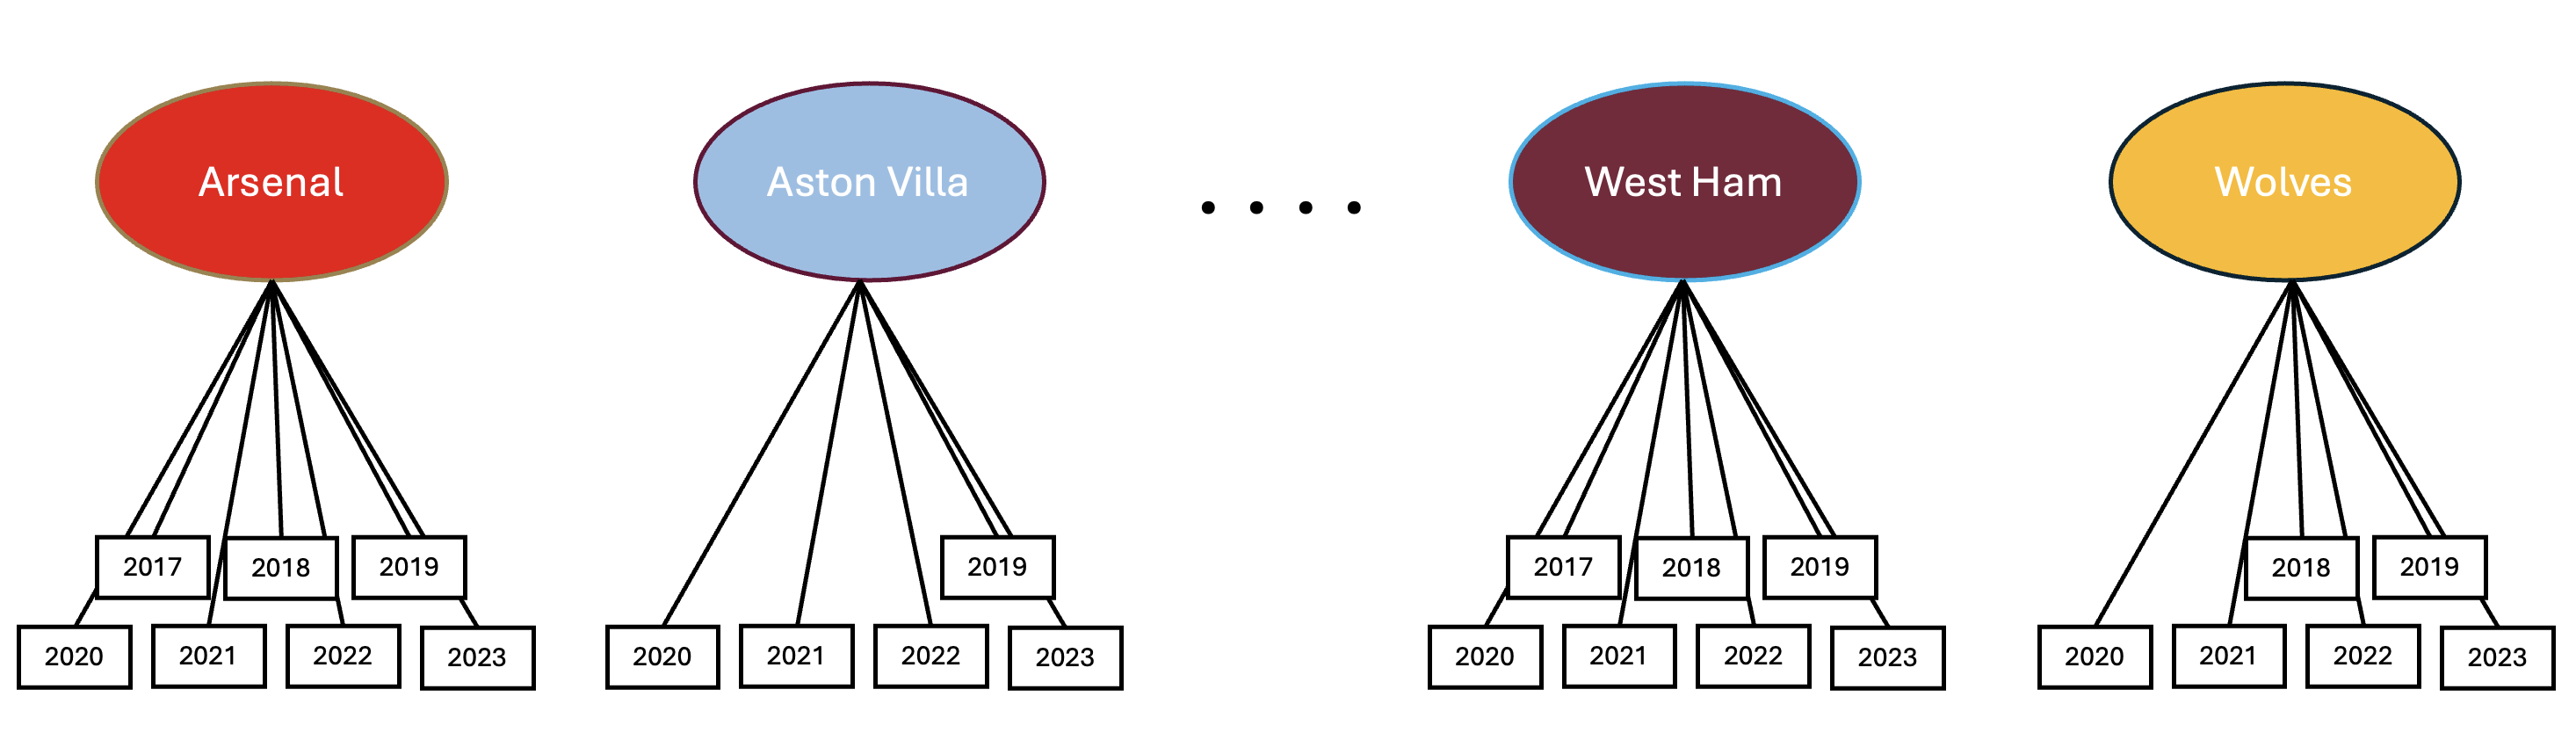
\includegraphics{images/multi_level_structure.png}

\subsubsection{Variable Chart}\label{variable-chart}

\begin{longtable}[]{@{}
  >{\raggedright\arraybackslash}p{(\columnwidth - 6\tabcolsep) * \real{0.3100}}
  >{\raggedright\arraybackslash}p{(\columnwidth - 6\tabcolsep) * \real{0.1500}}
  >{\raggedright\arraybackslash}p{(\columnwidth - 6\tabcolsep) * \real{0.1500}}
  >{\raggedright\arraybackslash}p{(\columnwidth - 6\tabcolsep) * \real{0.3700}}@{}}
\toprule\noalign{}
\begin{minipage}[b]{\linewidth}\raggedright
Name
\end{minipage} & \begin{minipage}[b]{\linewidth}\raggedright
Role
\end{minipage} & \begin{minipage}[b]{\linewidth}\raggedright
Type
\end{minipage} & \begin{minipage}[b]{\linewidth}\raggedright
Values
\end{minipage} \\
\midrule\noalign{}
\endhead
\bottomrule\noalign{}
\endlastfoot
Points & Response & Quantitative & \textgreater0 \\
Goals/90 & L1 Predictor & Quantitative & \textgreater0 \\
Goals Against/90 & L1 Predictor & Quantitative & \textgreater0 \\
Net Spend & L1 Predictor & Quantitative & -inf, inf \\
Average Net Spend (for team) & L2 Predictor & Quantitative & -inf,
inf \\
Luck Level & L1 Predictor & Categorical & (Lucky offense, Lucky
defense),

(Unlucky offense, Lucky defense),

(Lucky offense, Lucky defense),

(Unlucky offense, Unlucky defense) \\
\ldots{} & \ldots{} & \ldots{} & \ldots{} \\
Other ideas for L2 & & & \\
Team Cateogry & L2 Predictor & & Top 6, mid-table, relegation\ldots{} \\
& & & \\
\end{longtable}

\subsection{Part II: Exploratory Data
Analysis}\label{part-ii-exploratory-data-analysis}

\begin{Shaded}
\begin{Highlighting}[]
\CommentTok{\# Create a correlation plot to identify relationships between numeric variables}
\NormalTok{corr\_matrix }\OtherTok{\textless{}{-}}\NormalTok{ prem }\SpecialCharTok{\%\textgreater{}\%} 
  \FunctionTok{select}\NormalTok{(GF, GA, xG, xGA, Poss, Age, Sh, SoT, Dist, SoTA, CS, Expenditure, Arrivals, Income, Departures, Balance, Pts) }\SpecialCharTok{\%\textgreater{}\%} 
  \FunctionTok{cor}\NormalTok{()}
\FunctionTok{corrplot}\NormalTok{(corr\_matrix, }\AttributeTok{method =} \StringTok{"color"}\NormalTok{, }\AttributeTok{type =} \StringTok{"lower"}\NormalTok{, }\AttributeTok{tl.cex =} \FloatTok{0.7}\NormalTok{, }\AttributeTok{tl.pos =} \StringTok{"lt"}\NormalTok{)}\CommentTok{\#, addCoef.col = "black")}
\end{Highlighting}
\end{Shaded}

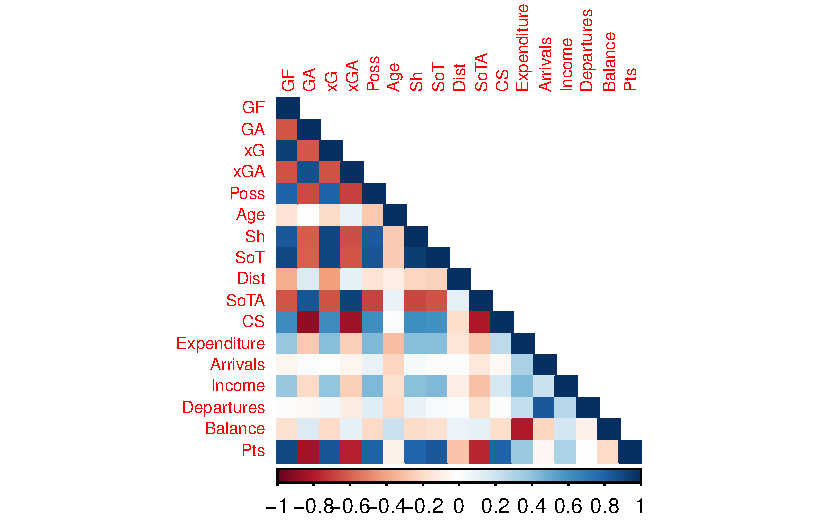
\includegraphics{project_part_3_files/figure-pdf/correlation-plot-1.pdf}

\begin{Shaded}
\begin{Highlighting}[]
\NormalTok{prem }\SpecialCharTok{\%\textgreater{}\%}
  \FunctionTok{ggplot}\NormalTok{() }\SpecialCharTok{+}
  \FunctionTok{geom\_point}\NormalTok{(}\FunctionTok{aes}\NormalTok{(}\AttributeTok{x =}\NormalTok{ GF, GA, }\AttributeTok{color =}\NormalTok{ Pts)) }\SpecialCharTok{+}
  \FunctionTok{theme\_bw}\NormalTok{() }\SpecialCharTok{+}
  \FunctionTok{theme}\NormalTok{(}\AttributeTok{plot.title.position =} \StringTok{"plot"}\NormalTok{) }\SpecialCharTok{+}
  \FunctionTok{labs}\NormalTok{(}\AttributeTok{x =} \StringTok{"Goals Scored per game"}\NormalTok{,}
       \AttributeTok{y =} \StringTok{"Goals Conceded per game"}\NormalTok{,}
       \AttributeTok{legend =} \StringTok{"Points"}\NormalTok{,}
       \AttributeTok{caption =} \StringTok{"Data from Fbref.com"}\NormalTok{,}
       \AttributeTok{title =} \StringTok{"Goals Scored and Goals Conceded vs Points"}\NormalTok{)}
\end{Highlighting}
\end{Shaded}

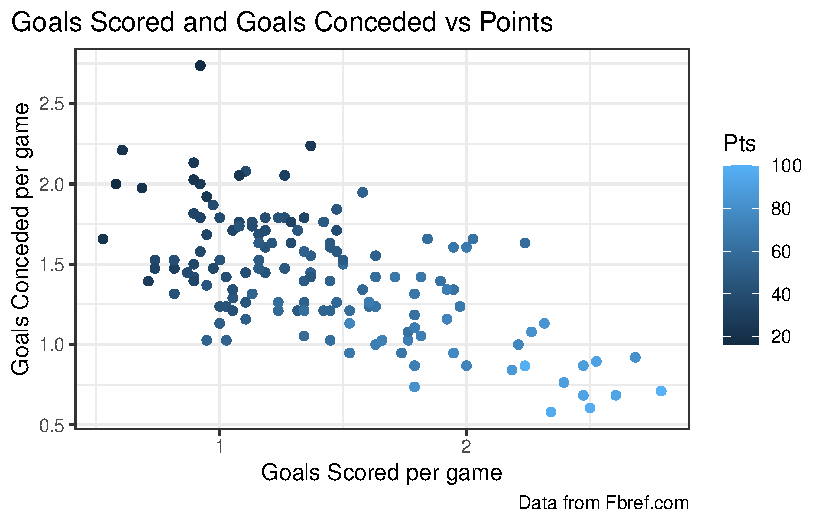
\includegraphics{project_part_3_files/figure-pdf/goals-and-points-plot-1.pdf}

\begin{Shaded}
\begin{Highlighting}[]
\NormalTok{prem }\SpecialCharTok{\%\textgreater{}\%}
  \FunctionTok{left\_join}\NormalTok{(prem\_colors, }\AttributeTok{by =} \StringTok{"Squad"}\NormalTok{) }\SpecialCharTok{\%\textgreater{}\%}
  \FunctionTok{ggplot}\NormalTok{() }\SpecialCharTok{+}
  \FunctionTok{geom\_point}\NormalTok{(}\FunctionTok{aes}\NormalTok{(}\AttributeTok{x =}\NormalTok{ Poss, }\AttributeTok{y =}\NormalTok{ Pts, }\AttributeTok{fill =}\NormalTok{ hex\_fill, }\AttributeTok{color =}\NormalTok{ hex\_color)) }\SpecialCharTok{+}
  \FunctionTok{theme\_bw}\NormalTok{() }\SpecialCharTok{+}
  \FunctionTok{scale\_fill\_identity}\NormalTok{() }\SpecialCharTok{+}
  \FunctionTok{scale\_color\_identity}\NormalTok{() }\SpecialCharTok{+}
  \FunctionTok{theme}\NormalTok{(}\AttributeTok{plot.title.position =} \StringTok{"plot"}\NormalTok{,}
        \AttributeTok{legend.position =} \StringTok{"none"}\NormalTok{) }\SpecialCharTok{+}
  \FunctionTok{labs}\NormalTok{(}\AttributeTok{y =} \StringTok{"Points"}\NormalTok{,}
       \AttributeTok{x =} \StringTok{"Average Possession (\%) over Season"}\NormalTok{,}
       \AttributeTok{caption =} \StringTok{"Data from Fbref.com"}\NormalTok{,}
       \AttributeTok{title =} \StringTok{"Team Posession vs Points"}\NormalTok{,}
       \AttributeTok{subtitle =} \StringTok{"Color by Team"}\NormalTok{)}
\end{Highlighting}
\end{Shaded}

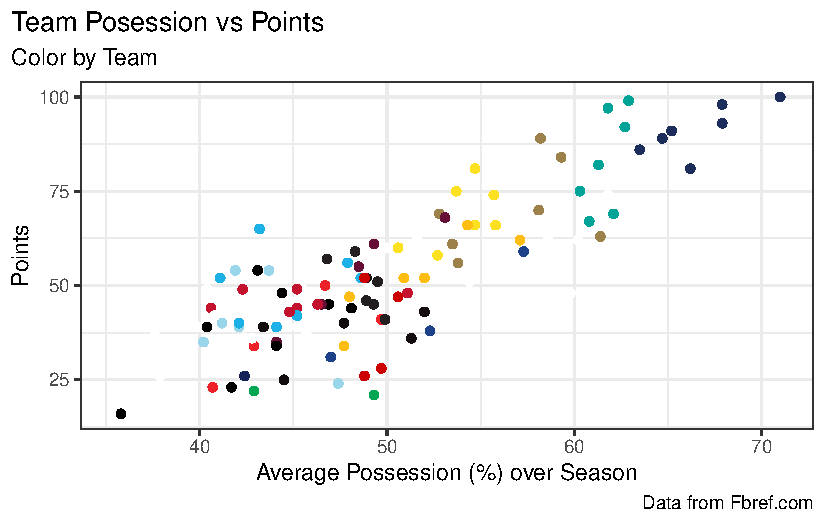
\includegraphics{project_part_3_files/figure-pdf/team-possession-plot-1.pdf}

\begin{Shaded}
\begin{Highlighting}[]
\CommentTok{\# Scatter plot for net spend vs point total}
\NormalTok{prem }\SpecialCharTok{\%\textgreater{}\%}
  \FunctionTok{left\_join}\NormalTok{(prem\_colors, }\AttributeTok{by =} \StringTok{"Squad"}\NormalTok{) }\SpecialCharTok{\%\textgreater{}\%}
  \FunctionTok{mutate}\NormalTok{(}\AttributeTok{label =} \FunctionTok{ifelse}\NormalTok{(Balance }\SpecialCharTok{\textless{}} \SpecialCharTok{{-}}\DecValTok{400}\NormalTok{, }\FunctionTok{paste0}\NormalTok{(Squad, }\StringTok{": "}\NormalTok{, Season), }\StringTok{""}\NormalTok{)) }\SpecialCharTok{\%\textgreater{}\%}
  \FunctionTok{ggplot}\NormalTok{(}\FunctionTok{aes}\NormalTok{(}\AttributeTok{x =}\NormalTok{ Balance, }\AttributeTok{y =}\NormalTok{ Pts)) }\SpecialCharTok{+}
    \FunctionTok{geom\_point}\NormalTok{(}\FunctionTok{aes}\NormalTok{(}\AttributeTok{color =}\NormalTok{ hex\_fill)) }\SpecialCharTok{+}
    \FunctionTok{geom\_text}\NormalTok{(}\FunctionTok{aes}\NormalTok{(}\AttributeTok{x =}\NormalTok{ Balance, }\AttributeTok{y =}\NormalTok{ Pts, }\AttributeTok{label =}\NormalTok{ label), }\AttributeTok{hjust =} \SpecialCharTok{{-}}\FloatTok{0.1}\NormalTok{, }\AttributeTok{color =} \StringTok{"\#034694"}\NormalTok{) }\SpecialCharTok{+}
    \FunctionTok{geom\_smooth}\NormalTok{(}\AttributeTok{method =} \StringTok{"lm"}\NormalTok{, }\AttributeTok{se =} \ConstantTok{FALSE}\NormalTok{, }\AttributeTok{color =} \StringTok{"red"}\NormalTok{) }\SpecialCharTok{+}
    \FunctionTok{labs}\NormalTok{(}\AttributeTok{title =} \StringTok{"Premier League Point Totals by Net Spend"}\NormalTok{,}
         \AttributeTok{subtitle =} \StringTok{"(2017{-}2023 Seasons)"}\NormalTok{,}
         \AttributeTok{caption =} \StringTok{"Data from Fbref.com \& Transfermarkt.com"}\NormalTok{,}
         \AttributeTok{x =} \StringTok{"Net Spend (in Million Euros)"}\NormalTok{,}
         \AttributeTok{y =} \StringTok{"Points"}\NormalTok{) }\SpecialCharTok{+}
  \FunctionTok{theme\_bw}\NormalTok{() }\SpecialCharTok{+}
  \FunctionTok{scale\_color\_identity}\NormalTok{() }\SpecialCharTok{+}
  \FunctionTok{theme}\NormalTok{(}
    \AttributeTok{plot.title.position =} \StringTok{"plot"}\NormalTok{,}
    \AttributeTok{plot.title =} \FunctionTok{element\_text}\NormalTok{(}\AttributeTok{size =} \DecValTok{12}\NormalTok{)}
\NormalTok{  )}
\end{Highlighting}
\end{Shaded}

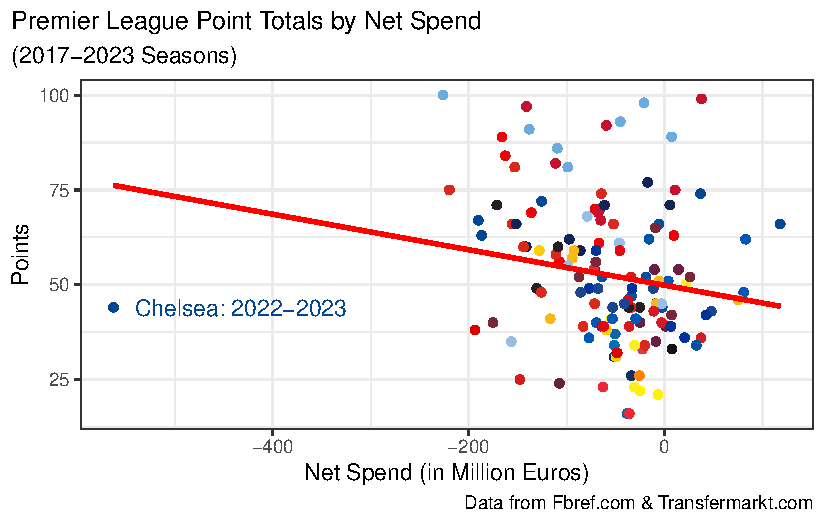
\includegraphics{project_part_3_files/figure-pdf/net-spend-vs-points-l1-1.pdf}

\begin{Shaded}
\begin{Highlighting}[]
\NormalTok{prem }\SpecialCharTok{\%\textgreater{}\%}
  \FunctionTok{group\_by}\NormalTok{(Squad) }\SpecialCharTok{\%\textgreater{}\%}
  \FunctionTok{summarize}\NormalTok{(}\AttributeTok{Mean\_Balance =} \SpecialCharTok{{-}}\DecValTok{1}\SpecialCharTok{*}\FunctionTok{mean}\NormalTok{(Balance),}
            \AttributeTok{Mean\_Pts =} \FunctionTok{mean}\NormalTok{(Pts)) }\SpecialCharTok{\%\textgreater{}\%}
\CommentTok{\# left\_join(prem \%\textgreater{}\% select(Squad, Pts), by = "Squad") \%\textgreater{}\%}
  \FunctionTok{left\_join}\NormalTok{(prem\_colors, }\AttributeTok{by =} \StringTok{"Squad"}\NormalTok{) }\SpecialCharTok{\%\textgreater{}\%}
  \FunctionTok{ggplot}\NormalTok{() }\SpecialCharTok{+}
  \FunctionTok{geom\_point}\NormalTok{(}\FunctionTok{aes}\NormalTok{(}\AttributeTok{x =}\NormalTok{ Mean\_Balance, }\AttributeTok{y =}\NormalTok{ Mean\_Pts, }\AttributeTok{fill =}\NormalTok{ hex\_fill, }\AttributeTok{color =}\NormalTok{ hex\_color)) }\SpecialCharTok{+}
  \FunctionTok{theme\_bw}\NormalTok{() }\SpecialCharTok{+}
  \FunctionTok{scale\_fill\_identity}\NormalTok{() }\SpecialCharTok{+}
  \FunctionTok{scale\_color\_identity}\NormalTok{() }\SpecialCharTok{+}
  \FunctionTok{theme}\NormalTok{(}\AttributeTok{plot.title.position =} \StringTok{"plot"}\NormalTok{) }\SpecialCharTok{+}
  \FunctionTok{labs}\NormalTok{(}\AttributeTok{title =} \StringTok{"Premier League Point Totals by Average Spend"}\NormalTok{,}
  \AttributeTok{subtitle =} \StringTok{"(2017{-}2023 Seasons)"}\NormalTok{,}
       \AttributeTok{caption =} \StringTok{"Data from Fbref.com \& Transfermarkt.com"}\NormalTok{,}
       \AttributeTok{x =} \StringTok{"Average Spend (in Million Euros)"}\NormalTok{,}
       \AttributeTok{y =} \StringTok{"Points"}\NormalTok{) }\SpecialCharTok{+}
  \FunctionTok{geom\_smooth}\NormalTok{(}\FunctionTok{aes}\NormalTok{(}\AttributeTok{x =}\NormalTok{ Mean\_Balance, }\AttributeTok{y =}\NormalTok{ Mean\_Pts), }\AttributeTok{method =} \StringTok{"lm"}\NormalTok{, }\AttributeTok{se =} \ConstantTok{FALSE}\NormalTok{, }\AttributeTok{color =} \StringTok{"red"}\NormalTok{)}
\end{Highlighting}
\end{Shaded}

\begin{verbatim}
`geom_smooth()` using formula = 'y ~ x'
\end{verbatim}

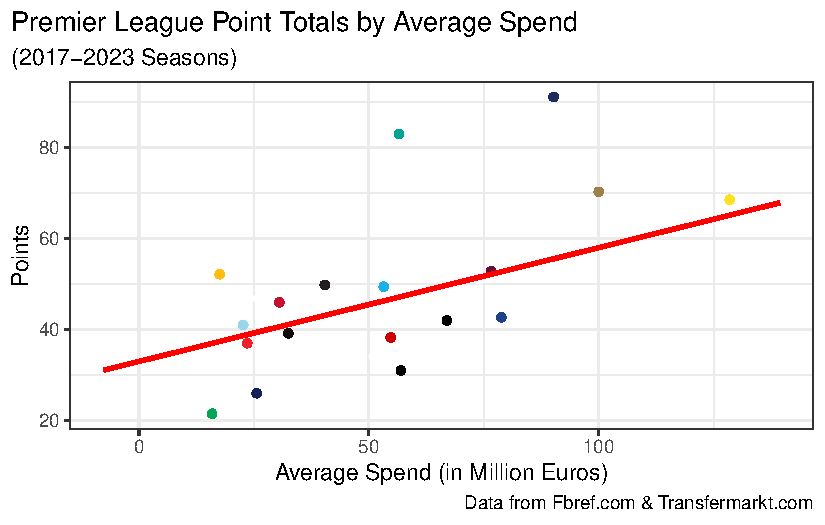
\includegraphics{project_part_3_files/figure-pdf/spend-by-team-l2-1.pdf}

\subsection{Part III: Modeling Results}\label{part-iii-modeling-results}

\subsubsection{Variability Across Teams (Level
2)}\label{variability-across-teams-level-2}

\begin{Shaded}
\begin{Highlighting}[]
\NormalTok{squad\_colors }\OtherTok{\textless{}{-}} \FunctionTok{read\_csv}\NormalTok{(here}\SpecialCharTok{::}\FunctionTok{here}\NormalTok{(}\StringTok{"data"}\NormalTok{, }\StringTok{"prem\_team\_colors.csv"}\NormalTok{), }\AttributeTok{show\_col\_types =} \ConstantTok{FALSE}\NormalTok{)}

\NormalTok{prem }\SpecialCharTok{\%\textgreater{}\%}
  \FunctionTok{left\_join}\NormalTok{(squad\_colors, }\AttributeTok{by =} \StringTok{"Squad"}\NormalTok{) }\SpecialCharTok{\%\textgreater{}\%}
  \FunctionTok{ggplot}\NormalTok{() }\SpecialCharTok{+}
  \FunctionTok{geom\_dotplot}\NormalTok{(}\FunctionTok{aes}\NormalTok{(}\AttributeTok{x =}\NormalTok{ Pts, }\AttributeTok{y =}\NormalTok{ Squad, }\AttributeTok{fill =}\NormalTok{ hex\_fill, }\AttributeTok{color =}\NormalTok{ hex\_color), }\AttributeTok{binwidth =} \DecValTok{1}\NormalTok{, }\AttributeTok{dotsize =}\NormalTok{ .}\DecValTok{75}\NormalTok{) }\SpecialCharTok{+}
  \FunctionTok{theme}\NormalTok{(}\AttributeTok{legend.position =} \StringTok{"none"}\NormalTok{) }\SpecialCharTok{+}
  \FunctionTok{scale\_fill\_identity}\NormalTok{() }\SpecialCharTok{+}
  \FunctionTok{scale\_color\_identity}\NormalTok{() }\SpecialCharTok{+}
  \FunctionTok{theme\_bw}\NormalTok{() }\SpecialCharTok{+}
  \FunctionTok{labs}\NormalTok{(}
    \AttributeTok{x =} \StringTok{"Points"}\NormalTok{,}
    \AttributeTok{y =} \StringTok{""}\NormalTok{,}
    \AttributeTok{title =} \StringTok{"Distribution of Points by Team (2017{-}2023 Seasons)"}\NormalTok{,}
    \AttributeTok{caption =} \StringTok{"Data from Fbref.com"}
\NormalTok{    ) }\SpecialCharTok{+}
  \FunctionTok{theme}\NormalTok{(}\AttributeTok{plot.title.position =} \StringTok{"plot"}\NormalTok{)}
\end{Highlighting}
\end{Shaded}

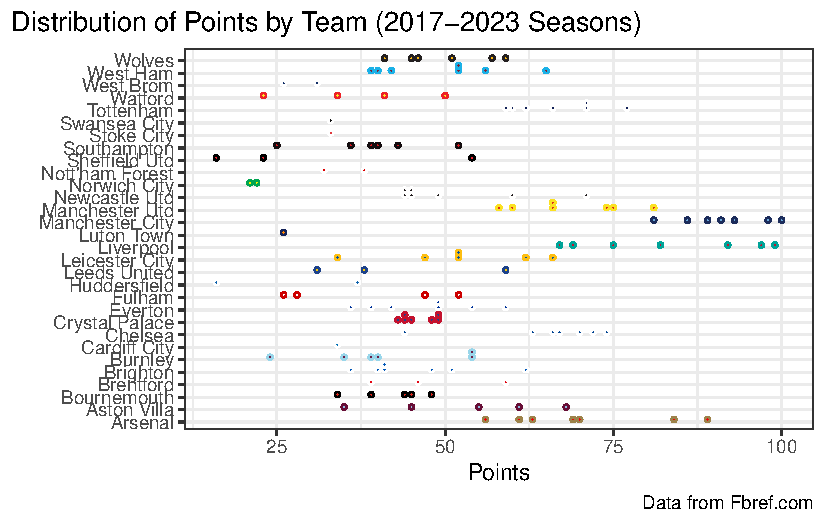
\includegraphics{project_part_3_files/figure-pdf/dot-plot-points-dist-1.pdf}

\begin{Shaded}
\begin{Highlighting}[]
\NormalTok{model00 }\OtherTok{\textless{}{-}} \FunctionTok{lm}\NormalTok{(Pts }\SpecialCharTok{\textasciitilde{}}\NormalTok{ Squad, }\AttributeTok{data =}\NormalTok{ prem)}
\FunctionTok{anova}\NormalTok{(model00)}
\end{Highlighting}
\end{Shaded}

\begin{verbatim}
Analysis of Variance Table

Response: Pts
           Df Sum Sq Mean Sq F value    Pr(>F)    
Squad      29  37233 1283.89  12.848 < 2.2e-16 ***
Residuals 110  10992   99.93                      
---
Signif. codes:  0 '***' 0.001 '**' 0.01 '*' 0.05 '.' 0.1 ' ' 1
\end{verbatim}

\subsubsection{Null Model}\label{null-model}

\begin{Shaded}
\begin{Highlighting}[]
\NormalTok{model0 }\OtherTok{\textless{}{-}} \FunctionTok{lmer}\NormalTok{(Pts }\SpecialCharTok{\textasciitilde{}} \DecValTok{1} \SpecialCharTok{+}\NormalTok{ (}\DecValTok{1} \SpecialCharTok{|}\NormalTok{ Squad), }\AttributeTok{data =}\NormalTok{ prem)}
\FunctionTok{summary}\NormalTok{(model0)}
\end{Highlighting}
\end{Shaded}

\begin{verbatim}
Linear mixed model fit by REML ['lmerMod']
Formula: Pts ~ 1 + (1 | Squad)
   Data: prem

REML criterion at convergence: 1108.9

Scaled residuals: 
     Min       1Q   Median       3Q      Max 
-2.02395 -0.60329 -0.08726  0.65915  2.11491 

Random effects:
 Groups   Name        Variance Std.Dev.
 Squad    (Intercept) 255.32   15.979  
 Residual              99.66    9.983  
Number of obs: 140, groups:  Squad, 30

Fixed effects:
            Estimate Std. Error t value
(Intercept)   47.388      3.091   15.33
\end{verbatim}

\subsubsection{Add Level 1 Vars}\label{add-level-1-vars}

\begin{Shaded}
\begin{Highlighting}[]
\NormalTok{model1 }\OtherTok{\textless{}{-}} \FunctionTok{lmer}\NormalTok{(Pts }\SpecialCharTok{\textasciitilde{}}\NormalTok{ GF }\SpecialCharTok{+}\NormalTok{ GA }\SpecialCharTok{+}\NormalTok{ (}\DecValTok{1} \SpecialCharTok{|}\NormalTok{ Squad), }\AttributeTok{data =}\NormalTok{ prem)}
\FunctionTok{summary}\NormalTok{(model1)}
\end{Highlighting}
\end{Shaded}

\begin{verbatim}
Linear mixed model fit by REML ['lmerMod']
Formula: Pts ~ GF + GA + (1 | Squad)
   Data: prem

REML criterion at convergence: 815.1

Scaled residuals: 
    Min      1Q  Median      3Q     Max 
-2.7861 -0.6433  0.0348  0.6699  3.2020 

Random effects:
 Groups   Name        Variance Std.Dev.
 Squad    (Intercept)  0.9551  0.9773  
 Residual             19.9221  4.4634  
Number of obs: 140, groups:  Squad, 30

Fixed effects:
            Estimate Std. Error t value
(Intercept)   49.474      3.024   16.36
GF            24.099      1.042   23.14
GA           -21.903      1.325  -16.54

Correlation of Fixed Effects:
   (Intr) GF    
GF -0.848       
GA -0.909  0.582
\end{verbatim}

\begin{Shaded}
\begin{Highlighting}[]
\NormalTok{model1\_1 }\OtherTok{\textless{}{-}} \FunctionTok{lmer}\NormalTok{(Pts }\SpecialCharTok{\textasciitilde{}}\NormalTok{ GF }\SpecialCharTok{+}\NormalTok{ GA }\SpecialCharTok{+}\NormalTok{ xG\_cat }\SpecialCharTok{+}\NormalTok{ (}\DecValTok{1} \SpecialCharTok{|}\NormalTok{ Squad), }\AttributeTok{data =}\NormalTok{ prem)}
\NormalTok{model1\_2}\OtherTok{\textless{}{-}} \FunctionTok{lmer}\NormalTok{(Pts }\SpecialCharTok{\textasciitilde{}}\NormalTok{ GF }\SpecialCharTok{+}\NormalTok{ GA }\SpecialCharTok{+}\NormalTok{ xG\_diff }\SpecialCharTok{+}\NormalTok{ xGA\_diff }\SpecialCharTok{+}\NormalTok{ (}\DecValTok{1} \SpecialCharTok{|}\NormalTok{ Squad), }\AttributeTok{data =}\NormalTok{ prem)}
\NormalTok{model1\_3}\OtherTok{\textless{}{-}} \FunctionTok{lmer}\NormalTok{(Pts }\SpecialCharTok{\textasciitilde{}}\NormalTok{ GF }\SpecialCharTok{+}\NormalTok{ GA }\SpecialCharTok{+}\NormalTok{ Balance }\SpecialCharTok{+}\NormalTok{ (}\DecValTok{1} \SpecialCharTok{|}\NormalTok{ Squad), }\AttributeTok{data =}\NormalTok{ prem)}
\NormalTok{model1\_4}\OtherTok{\textless{}{-}} \FunctionTok{lmer}\NormalTok{(Pts }\SpecialCharTok{\textasciitilde{}}\NormalTok{ GF }\SpecialCharTok{+}\NormalTok{ GA }\SpecialCharTok{+}\NormalTok{ SoT\_diff }\SpecialCharTok{+}\NormalTok{ (}\DecValTok{1} \SpecialCharTok{|}\NormalTok{ Squad), }\AttributeTok{data =}\NormalTok{ prem)}
\end{Highlighting}
\end{Shaded}

\begin{Shaded}
\begin{Highlighting}[]
\FunctionTok{anova}\NormalTok{(model1, model1\_1)}
\end{Highlighting}
\end{Shaded}

\begin{verbatim}
refitting model(s) with ML (instead of REML)
\end{verbatim}

\begin{verbatim}
Data: prem
Models:
model1: Pts ~ GF + GA + (1 | Squad)
model1_1: Pts ~ GF + GA + xG_cat + (1 | Squad)
         npar    AIC    BIC  logLik deviance  Chisq Df Pr(>Chisq)
model1      5 829.01 843.72 -409.51   819.01                     
model1_1    8 834.59 858.13 -409.30   818.59 0.4193  3     0.9362
\end{verbatim}

\begin{Shaded}
\begin{Highlighting}[]
\FunctionTok{cat}\NormalTok{(}\StringTok{"}\SpecialCharTok{\textbackslash{}n\textbackslash{}n}\StringTok{"}\NormalTok{)}
\end{Highlighting}
\end{Shaded}

\begin{Shaded}
\begin{Highlighting}[]
\FunctionTok{anova}\NormalTok{(model1, model1\_2)}
\end{Highlighting}
\end{Shaded}

\begin{verbatim}
refitting model(s) with ML (instead of REML)
\end{verbatim}

\begin{verbatim}
Data: prem
Models:
model1: Pts ~ GF + GA + (1 | Squad)
model1_2: Pts ~ GF + GA + xG_diff + xGA_diff + (1 | Squad)
         npar    AIC    BIC  logLik deviance  Chisq Df Pr(>Chisq)
model1      5 829.01 843.72 -409.51   819.01                     
model1_2    7 829.80 850.39 -407.90   815.80 3.2098  2     0.2009
\end{verbatim}

\begin{Shaded}
\begin{Highlighting}[]
\FunctionTok{cat}\NormalTok{(}\StringTok{"}\SpecialCharTok{\textbackslash{}n\textbackslash{}n}\StringTok{"}\NormalTok{)}
\end{Highlighting}
\end{Shaded}

\begin{Shaded}
\begin{Highlighting}[]
\FunctionTok{anova}\NormalTok{(model1, model1\_3)}
\end{Highlighting}
\end{Shaded}

\begin{verbatim}
refitting model(s) with ML (instead of REML)
\end{verbatim}

\begin{verbatim}
Data: prem
Models:
model1: Pts ~ GF + GA + (1 | Squad)
model1_3: Pts ~ GF + GA + Balance + (1 | Squad)
         npar    AIC    BIC  logLik deviance  Chisq Df Pr(>Chisq)
model1      5 829.01 843.72 -409.51   819.01                     
model1_3    6 830.49 848.14 -409.24   818.49 0.5227  1     0.4697
\end{verbatim}

\begin{Shaded}
\begin{Highlighting}[]
\FunctionTok{cat}\NormalTok{(}\StringTok{"}\SpecialCharTok{\textbackslash{}n\textbackslash{}n}\StringTok{"}\NormalTok{)}
\end{Highlighting}
\end{Shaded}

\begin{Shaded}
\begin{Highlighting}[]
\FunctionTok{anova}\NormalTok{(model1, model1\_4)}
\end{Highlighting}
\end{Shaded}

\begin{verbatim}
refitting model(s) with ML (instead of REML)
\end{verbatim}

\begin{verbatim}
Data: prem
Models:
model1: Pts ~ GF + GA + (1 | Squad)
model1_4: Pts ~ GF + GA + SoT_diff + (1 | Squad)
         npar    AIC    BIC  logLik deviance  Chisq Df Pr(>Chisq)
model1      5 829.01 843.72 -409.51   819.01                     
model1_4    6 830.95 848.60 -409.48   818.95 0.0617  1     0.8039
\end{verbatim}

\subsubsection{Add Level 2 Vars}\label{add-level-2-vars}

\begin{Shaded}
\begin{Highlighting}[]
\NormalTok{prem }\OtherTok{\textless{}{-}}\NormalTok{ prem }\SpecialCharTok{\%\textgreater{}\%}
  \FunctionTok{left\_join}\NormalTok{(prem }\SpecialCharTok{\%\textgreater{}\%}
              \FunctionTok{group\_by}\NormalTok{(Squad) }\SpecialCharTok{\%\textgreater{}\%}
              \FunctionTok{summarize}\NormalTok{(}\AttributeTok{Balance\_mean =} \SpecialCharTok{{-}}\DecValTok{1}\SpecialCharTok{*}\FunctionTok{mean}\NormalTok{(Balance)),}
            \AttributeTok{by =} \StringTok{"Squad"}
\NormalTok{  )}
\end{Highlighting}
\end{Shaded}

\begin{Shaded}
\begin{Highlighting}[]
\NormalTok{model2 }\OtherTok{\textless{}{-}} \FunctionTok{lmer}\NormalTok{(Pts }\SpecialCharTok{\textasciitilde{}}\NormalTok{ GF }\SpecialCharTok{+}\NormalTok{ GA }\SpecialCharTok{+}\NormalTok{ Balance\_mean }\SpecialCharTok{+}\NormalTok{ (}\DecValTok{1} \SpecialCharTok{|}\NormalTok{ Squad), }\AttributeTok{data =}\NormalTok{ prem)}
\end{Highlighting}
\end{Shaded}

\begin{verbatim}
boundary (singular) fit: see help('isSingular')
\end{verbatim}

\begin{Shaded}
\begin{Highlighting}[]
\FunctionTok{summary}\NormalTok{(model2)}
\end{Highlighting}
\end{Shaded}

\begin{verbatim}
Linear mixed model fit by REML ['lmerMod']
Formula: Pts ~ GF + GA + Balance_mean + (1 | Squad)
   Data: prem

REML criterion at convergence: 815.9

Scaled residuals: 
    Min      1Q  Median      3Q     Max 
-2.8271 -0.6048  0.1171  0.6113  3.4867 

Random effects:
 Groups   Name        Variance Std.Dev.
 Squad    (Intercept)  0.00    0.000   
 Residual             19.96    4.467   
Number of obs: 140, groups:  Squad, 30

Fixed effects:
              Estimate Std. Error t value
(Intercept)   49.11412    2.95766  16.606
GF            23.03892    1.05930  21.749
GA           -21.86604    1.29747 -16.853
Balance_mean   0.03120    0.01181   2.643

Correlation of Fixed Effects:
            (Intr) GF     GA    
GF          -0.769              
GA          -0.919  0.557       
Balance_men -0.087 -0.362  0.056
optimizer (nloptwrap) convergence code: 0 (OK)
boundary (singular) fit: see help('isSingular')
\end{verbatim}

\subsubsection{Fit Random Slopes}\label{fit-random-slopes}

\subsubsection{Trying Longitudinal
Models}\label{trying-longitudinal-models}

\begin{Shaded}
\begin{Highlighting}[]
\NormalTok{model0 }\OtherTok{\textless{}{-}} \FunctionTok{lmer}\NormalTok{(Pts }\SpecialCharTok{\textasciitilde{}} \DecValTok{1} \SpecialCharTok{+}\NormalTok{ Season }\SpecialCharTok{+}\NormalTok{ (}\DecValTok{1} \SpecialCharTok{|}\NormalTok{ Squad), }\AttributeTok{data =}\NormalTok{ prem)}
\FunctionTok{summary}\NormalTok{(model0)}
\end{Highlighting}
\end{Shaded}

\begin{verbatim}
Linear mixed model fit by REML ['lmerMod']
Formula: Pts ~ 1 + Season + (1 | Squad)
   Data: prem

REML criterion at convergence: 1084.8

Scaled residuals: 
    Min      1Q  Median      3Q     Max 
-1.8427 -0.6395 -0.1172  0.5967  2.1021 

Random effects:
 Groups   Name        Variance Std.Dev.
 Squad    (Intercept) 258.5    16.08   
 Residual             104.0    10.20   
Number of obs: 140, groups:  Squad, 30

Fixed effects:
                Estimate Std. Error t value
(Intercept)      48.3860     3.7996  12.734
Season2018-2019   0.3077     3.3531   0.092
Season2019-2020  -1.0911     3.3739  -0.323
Season2020-2021  -1.0521     3.3785  -0.311
Season2021-2022  -1.7493     3.3960  -0.515
Season2022-2023  -2.4091     3.4173  -0.705
Season2023-2024  -1.2154     3.4565  -0.352

Correlation of Fixed Effects:
            (Intr) S2018- S2019- S2020- S2021- S2022-
Ss2018-2019 -0.439                                   
Ss2019-2020 -0.440  0.512                            
Ss2020-2021 -0.441  0.507  0.522                     
Ss2021-2022 -0.443  0.509  0.533  0.524              
Ss2022-2023 -0.446  0.512  0.521  0.528  0.532       
Ss2023-2024 -0.453  0.507  0.522  0.523  0.519  0.539
\end{verbatim}




\end{document}
